\section{eo\-Factory$<$ EOClass $>$ Class Template Reference}
\label{classeo_factory}\index{eoFactory@{eoFactory}}
{\bf EO}{\rm (p.\,\pageref{class_e_o})} Factory.  


{\tt \#include $<$eo\-Factory.h$>$}

Inheritance diagram for eo\-Factory$<$ EOClass $>$::\begin{figure}[H]
\begin{center}
\leavevmode
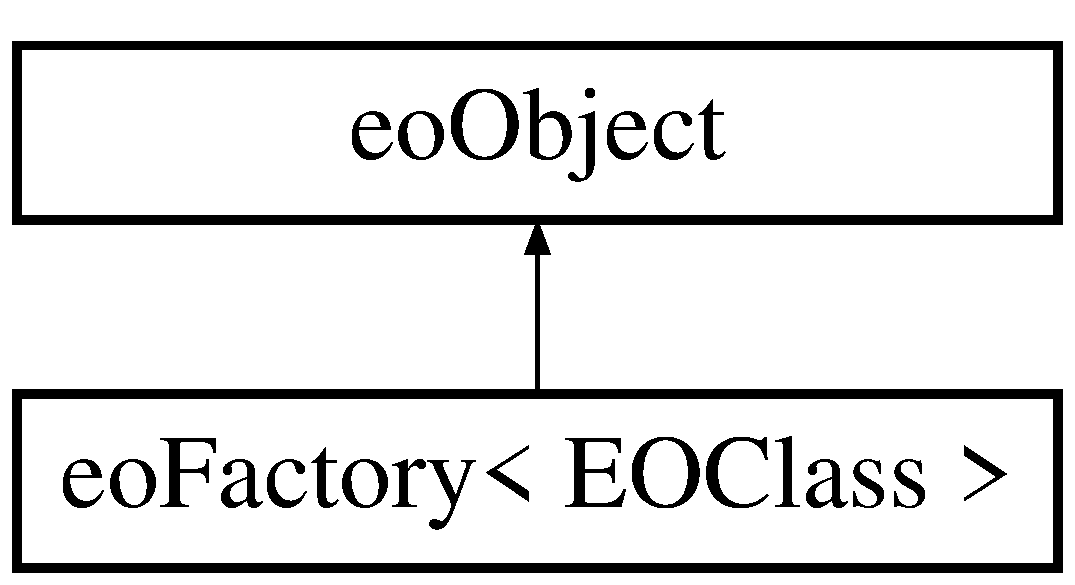
\includegraphics[height=2cm]{classeo_factory}
\end{center}
\end{figure}
\subsection*{Public Member Functions}
\begin{CompactItemize}
\item 
virtual EOClass $\ast$ {\bf make} (std::istream \&\_\-is)=0
\begin{CompactList}\small\item\em Another factory methods: creates an object from an std::istream, reading from it whatever is needed to create the object. \item\end{CompactList}\end{CompactItemize}
\begin{Indent}{\bf ctors and dtors}\par
\begin{CompactItemize}
\item 
{\bf eo\-Factory} ()\label{classeo_factory_z11_0}

\begin{CompactList}\small\item\em constructor \item\end{CompactList}\item 
virtual {\bf $\sim$eo\-Factory} ()\label{classeo_factory_z11_1}

\begin{CompactList}\small\item\em destructor \item\end{CompactList}\end{CompactItemize}
\end{Indent}
\begin{Indent}{\bf eo\-Object methods}\par
\begin{CompactItemize}
\item 
virtual std::string {\bf class\-Name} () const \label{classeo_factory_z13_0}

\begin{CompactList}\small\item\em Return the class id. \item\end{CompactList}\end{CompactItemize}
\end{Indent}


\subsection{Detailed Description}
\subsubsection*{template$<$class EOClass$>$ class eo\-Factory$<$ EOClass $>$}

{\bf EO}{\rm (p.\,\pageref{class_e_o})} Factory. 

A factory is used to create other objects. In particular, it can be used so that objects of that kind can180t be created in any other way. It should be instantiated with anything that needs a factory, like selectors or whatever; but the instance class should be the parent class from which all the object that are going to be created descend. This class basically defines an interface, as usual. The base factory class for each hierarchy should be redefined every time a new object is added to the hierarchy, which is not too good, but in any case, some code would have to be modified 



Definition at line 42 of file eo\-Factory.h.

\subsection{Member Function Documentation}
\index{eoFactory@{eo\-Factory}!make@{make}}
\index{make@{make}!eoFactory@{eo\-Factory}}
\subsubsection{\setlength{\rightskip}{0pt plus 5cm}template$<$class EOClass$>$ virtual EOClass$\ast$ {\bf eo\-Factory}$<$ EOClass $>$::make (std::istream \& {\em \_\-is})\hspace{0.3cm}{\tt  [pure virtual]}}\label{classeo_factory_a0}


Another factory methods: creates an object from an std::istream, reading from it whatever is needed to create the object. 

Usually, the format for the std::istream will be$\backslash$ object\-Type parameter1 parameter2 ... parametern$\backslash$

Implemented in {\bf eo\-Op\-Sel\-Mason$<$ eo\-Class $>$} {\rm (p.\,\pageref{classeo_op_sel_mason_a0})}, {\bf eo\-Select\-Factory$<$ EOT $>$} {\rm (p.\,\pageref{classeo_select_factory_a0})}, and {\bf eo\-Bit\-Op\-Factory$<$ EOT $>$} {\rm (p.\,\pageref{classeo_bit_op_factory_a0})}.

Referenced by eo\-Bit\-Op\-Factory$<$ EOT $>$::make().

The documentation for this class was generated from the following file:\begin{CompactItemize}
\item 
eo\-Factory.h\end{CompactItemize}
